\section{SwitchCrypt Design} \label{sec:design}

\subsection{SwitchCrypt Overview} \label{subsec:overview}

\begin{figure}[t]
   \centering
   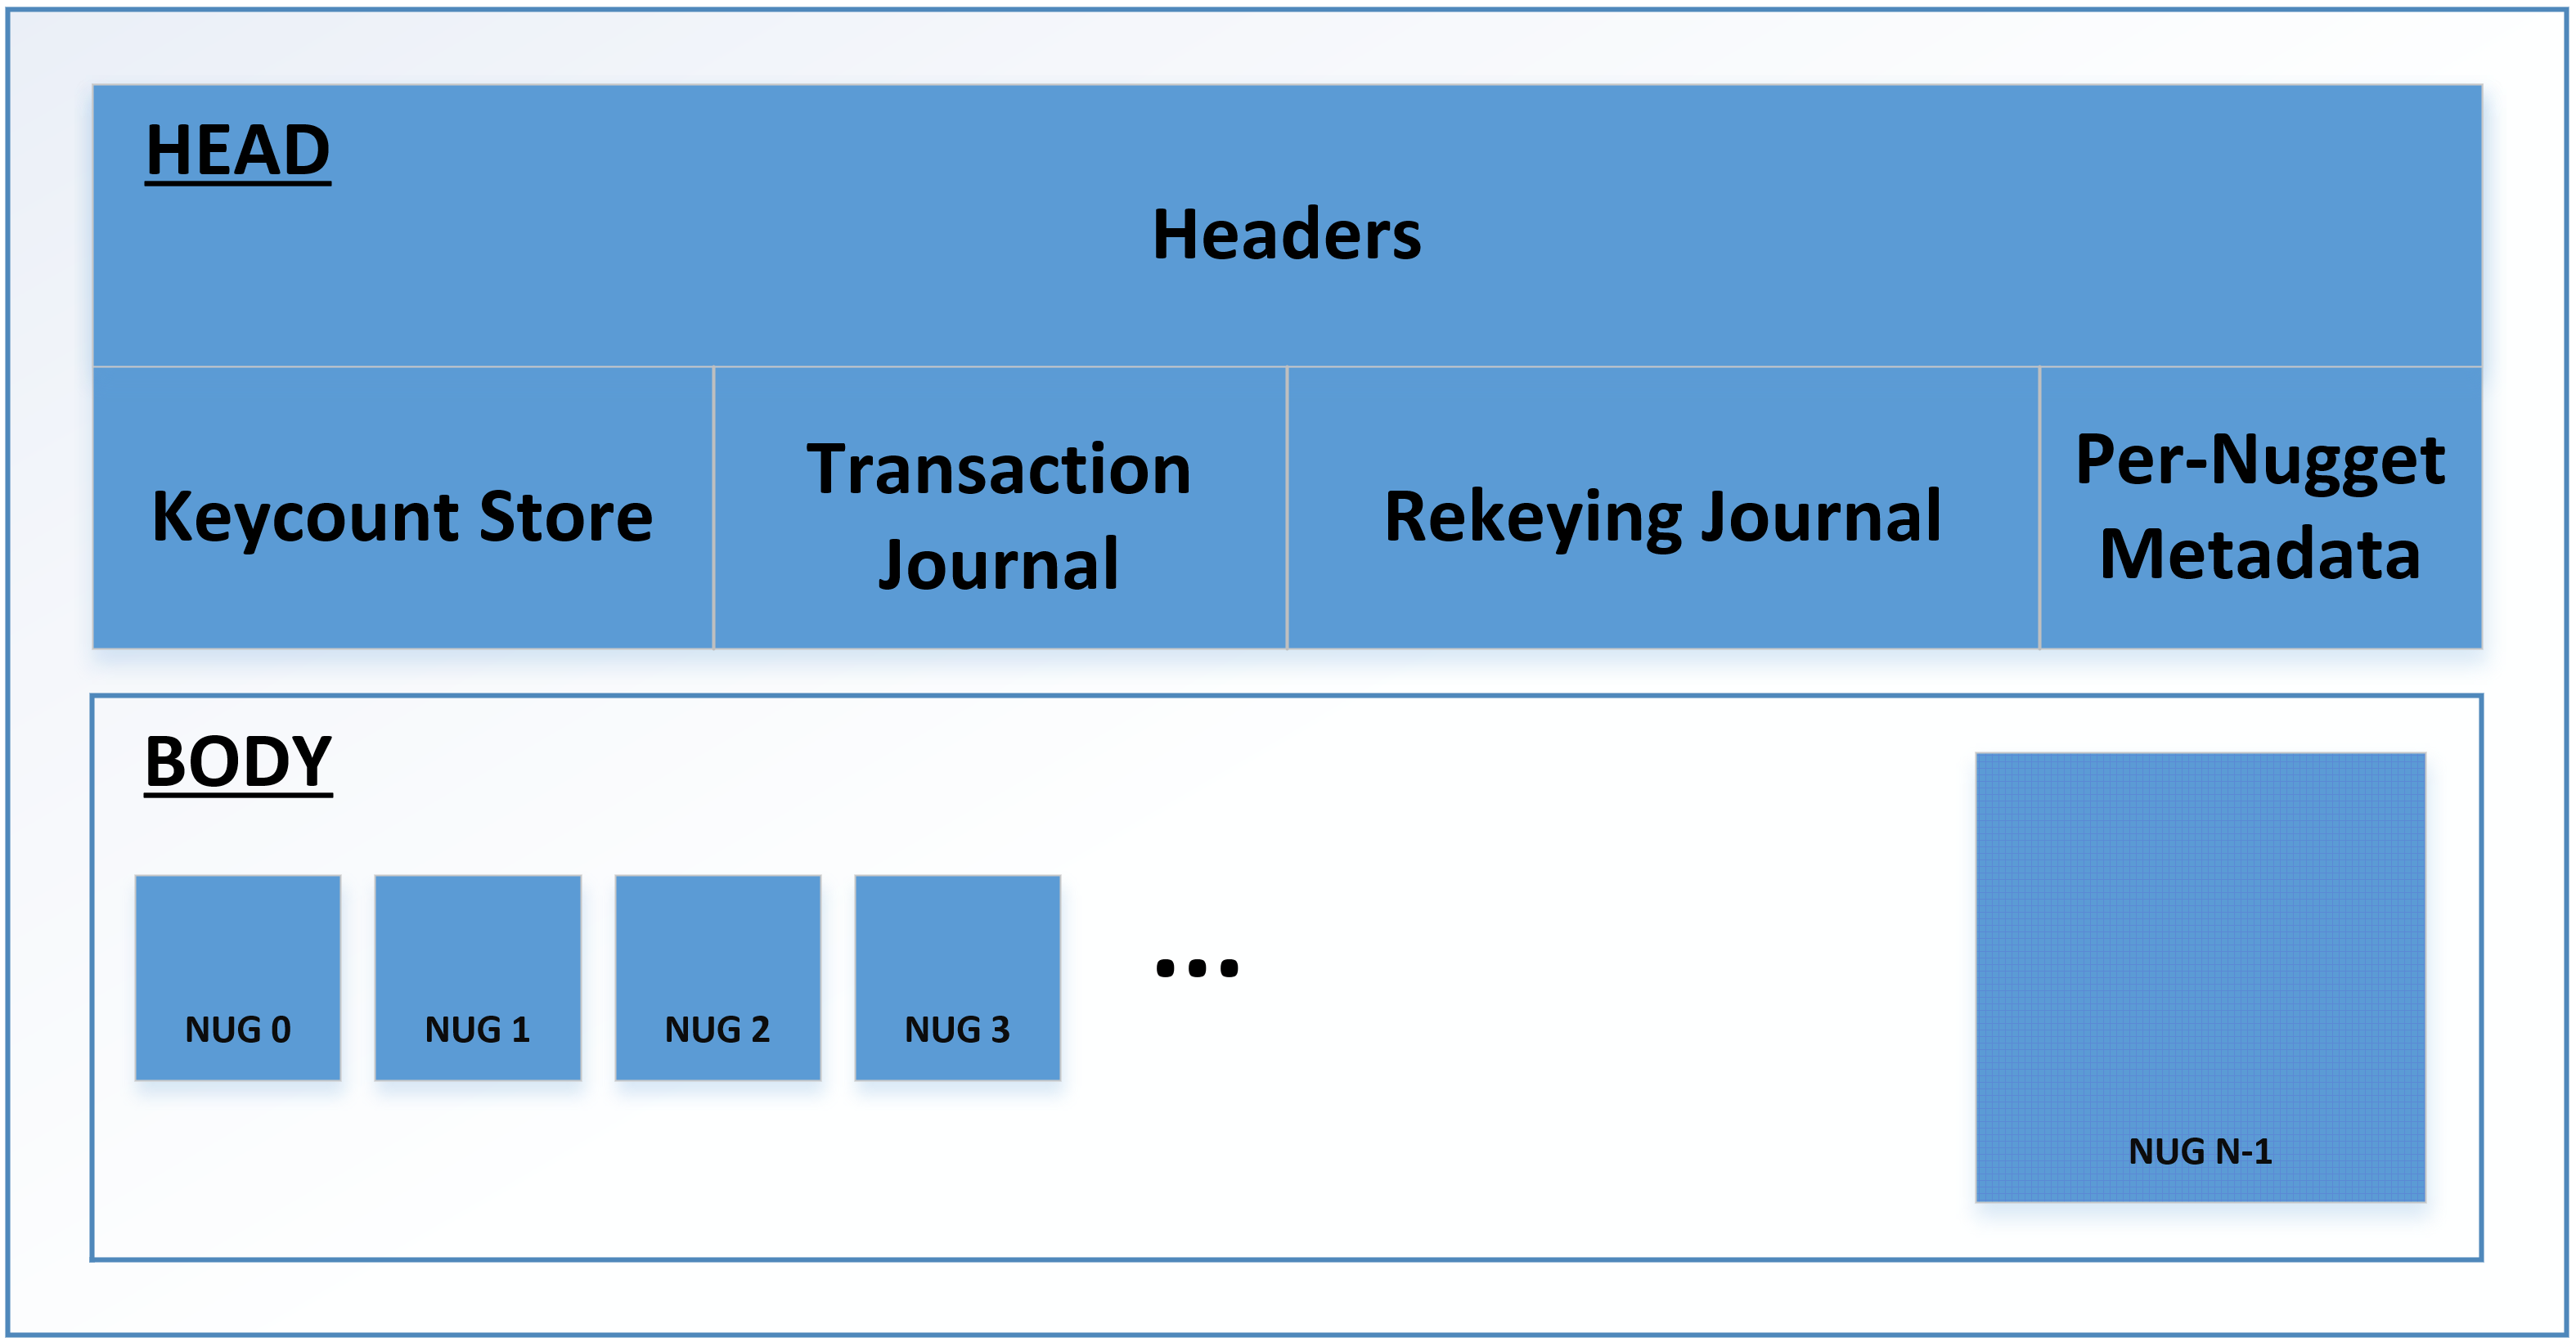
\includegraphics[width=\linewidth]{backstore.png}
   \caption{Layout of SwitchCrypt's drive layout.}\label{fig:backstore}
\end{figure}

SwitchCrypt consists of a \emph{Generic Stream Cipher Interface} and
\emph{Cryptographic Driver}; SwitchCrypt sits between a Log-structured File
System (LFS) on the OS and the underlying drive (backing storage) and device
controller (e.g. Flash Translation Layer). This is illustrated in
\figref{overview}, which provides an overview of the SwitchCrypt system design.

\begin{figure}[ht]
   \centering
   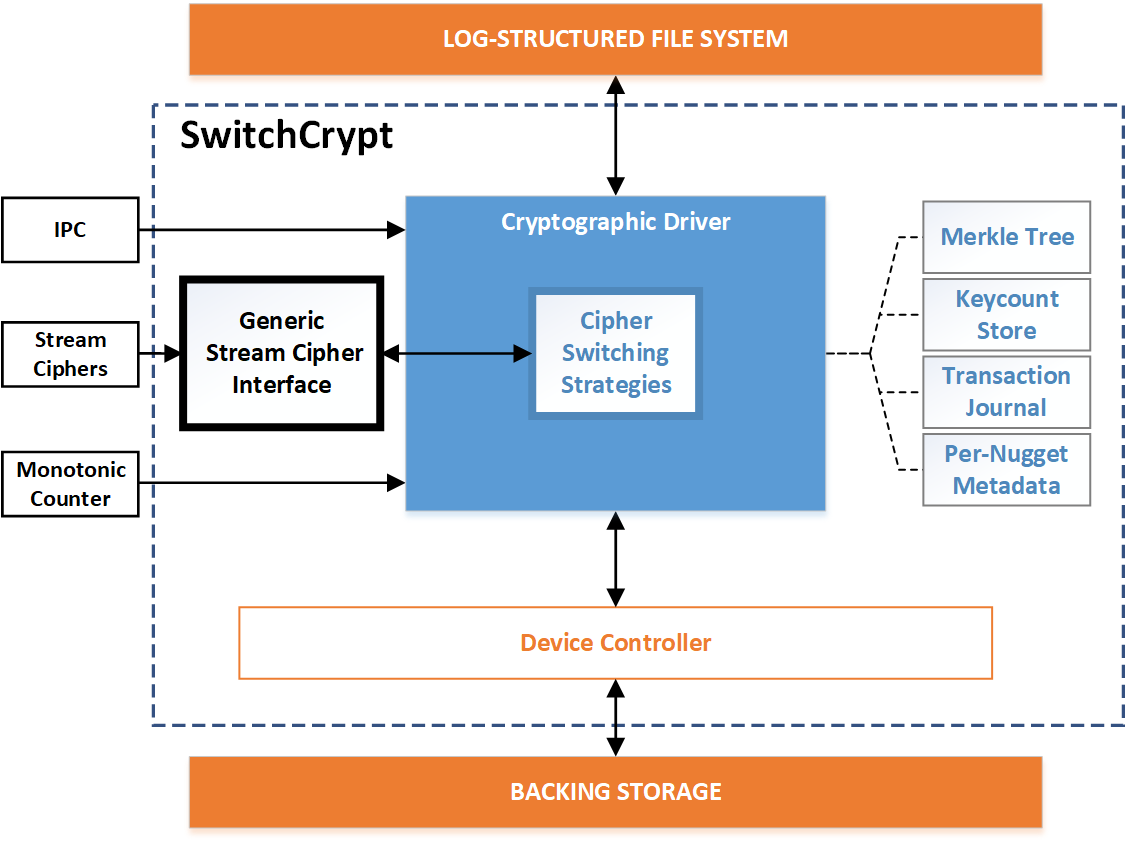
\includegraphics[width=\linewidth]{overview.png}
   \caption{Overview of the SwitchCrypt construction.}\label{fig:overview}
\end{figure}

The drive itself is divided into a \emph{HEAD} section and \emph{BODY} section
upon initialization, illustrated in \figref{backstore}. The HEAD consists of
metadata headers written during initialization~\cite{StrongBox} along with the
\emph{Keycount Store}, \emph{Transaction Journal}, \emph{Rekeying Journal}, and
\emph{Per-Nugget Metadata}, each drive-backed. These components are used by the
\emph{Cryptographic Driver} together with the \emph{Cipher Switching Strategy}
implementations to enable efficient per-unit cipher switching.

The BODY consists of a series independent same-size logical units called
\emph{nuggets}. A nugget consists of one or more contiguous physical drive
blocks. Each nugget is coupled with metadata in the HEAD indicating which cipher
was used to encrypt the nugget along with any additional ciphertext output; the
latter allows us to treat any non-length-preserving ciphers as if they were
length-preserving. SwitchCrypt uses the Keycount Store and Transaction Journal
components along with our nugget layout to 1) track, detect, and handle
overwrites, 2) limit the maximum length of any plaintext input to ciphers, thus
amortizing the overhead incurred during encryption, and 3) independently and
efficiently switch the cipher used to encrypt individual nuggets.

See Dickens et al.~\cite{StrongBox} for further discussion on handling
overwrites, preventing rollback attacks, and limiting plaintext length using the
nugget layout and aforesaid components. In the remainder of this section, we
detail the primary components of the SwitchCrypt design: how we quantify the
properties traded off between configurations (\cref{subsec:quantify}), the
Generic Stream Cipher Interface and Per-Nugget Metadata components
(\cref{subsec:interface}) which decouple cipher implementations from the
encryption process, and our Cipher Switching Strategy implementations
(\cref{subsec:strategies}) used to efficiently encrypt nuggets with different
ciphers.

\subsection{Quantifying Cipher Security Properties} \label{subsec:quantify}

To reason about when to trade off between the ciphers evaluated in this work, we
must have a way to quantitatively compare ciphers' utility for SwitchCrypt FDE.
However, different ciphers have a wide range of security properties, performance
profiles, and output characteristics. To address this need, we propose the
following framework for evaluating ciphers for SwitchCrypt FDE (see:
\tblref{security-quant}). Our framework is composed of three features: relative
round count, ciphertext randomization, and ciphertext expansion.

\begin{table}[]
   \begin{tabular}{@{}lllll@{}}
   \toprule
   \textbf{Cipher} & \textbf{RR} & \textbf{CR} & \textbf{CE} \\ \midrule
   ChaCha8         & 0           & 0           & 1           \\
   ChaCha12        & 0.5         & 0           & 1           \\
   ChaCha20        & 1           & 0           & 1           \\
   Salsa8          & 0           & 0           & 1           \\
   Salsa12         & 0.5         & 0           & 1           \\
   Salsa20         & 1           & 0           & 1           \\
   HC128           & 0           & 0           & 1           \\
   HC256           & 1           & 0           & 1           \\
   Freestyle (F)   & 0           & 1           & 0           \\
   Freestyle (B)   & 0.5         & 2           & 0           \\
   Freestyle (S)   & 1           & 3           & 0           \\
\end{tabular}
   \caption{\TODO{caption here}}
   \label{tbl:security-quant}
 \end{table}

\subsubsection{Relative Rounds (RR)}

The ciphers we examine in this paper are all constructed around the notion of
\emph{rounds}, where a higher number of rounds or longer key is positively
correlated with a higher resistance to brute force given no fatal related-key
attacks. This feature represents how many rounds the cipher executes compared to
the accepted ``standard'' round count for that cipher. For instance: ChaCha8 is
a reduced round version of the standard ChaCha20, both using 256-bit keys.

\TODO{Include the following? Work it in: a cipher with standard resistance to
brute force and offline/dictionary attacks has no kind of \emph{key-guessing
penalty}~\cite{Freestyle}---the ciphertext is decrypted no slower when given the
incorrect key versus the correct key.}

\subsubsection{Ciphertext Randomization (CR)}

A cipher with output randomization generates different ciphertexts
non-\\deterministically given the same key, nonce, and message. This makes
chosen-ciphertext (CCA) and other attacks where the ciphertext is in full
control of the adversary much more difficult~\cite{Freestyle}.

This is a binary feature in that a cipher either outputs deterministically given
the same input or it does not. A cipher with non-deterministic output given the
same key, nonce, and message as inputs scores a 1 for this feature while a
cipher with deterministic output given the same input scores a 0.

\subsubsection{Ciphertext Expansion (CE)}

It's binary. Words.

\subsection{Generic Stream Cipher Interface} \label{subsec:interface}

There are \emph{many} ciphers we might use with SwitchCrypt, each with various
input requirements and output considerations. A key difference with prior work
is that SwitchCrypt must be able to encrypt and decrypt arbitrary nuggets
without worrying about a cipher's implementation details; prior approaches could
have cipher-specific implementations because they did not consider switching.
Thus, the cipher-specific details must be handled with care or security is
violated. With our novel cipher interface, we present an interface that
\emph{decouples} cipher implementations from the encryption/decryption process.
This allows any cipher to be integrated into SwitchCrypt without modification or
special considerations. Hence, different stream ciphers become interchangeable
when they would normally be incompatible, preventing us from trading them off
one another.

The interface is accessible at three levels:

\begin{enumerate}
   \item \textbf{\texttt{crypt\_data}}\\\texttt{crypt\_data} operates at a
   fine-grain level independent of SwitchCrypt's internals. Implementations
   receive an index and offset and are expected to return some number of bytes,
   \ie{a keystream}, which is XORed with nugget contents. At this level, there
   is no distinction made between encryption and decryption since both are
   accomplished with a simple XOR. This interface level has the lowest
   implementation overhead and least flexibility.

   \item \textbf{\texttt{crypt\_data\_low}}\\\texttt{crypt\_data\_low}
   is identical to \texttt{crypt\_data} but provides a slightly lower level of
   abstraction when accessing the backing store, giving implementations more
   control over the XORing process. This is useful for less flexible ciphers but
   comes at the cost of increased implementation overhead.

   \item \textbf{\texttt{read\_data}} and \textbf{\texttt{write\_data}}\\
   These operate at a coarse-grain level tightly integrated with SwitchCrypt
   internals. Implementations are expected to handle all stages of cipher
   switching manually. Unlike the other two levels, encryption and decryption
   are distinct concerns. \texttt{read\_data} handles decryption during reads.
   \texttt{write\_data} handles encryption during writes. In exchange for
   maximum flexibility, there is significant implementation overhead with this
   approach.
\end{enumerate}

Were we using simple ciphers exclusively, \ie{those that do not differentiate
between encryption and decryption and always produce output of the same length
as the input}, we could generate a keystream and XOR it with data without the
the need for a new a interface. However, some cipher implementations treat
encryption and decryption as two distinct operations. Others require different
parameters or special considerations before XORing the keystream with data.
Others produce extra output that must be stored during encryption and fetched
during decryption. Others exhibit some combination of these concerns. Our
interface presents the cryptographic driver with a single unified interface
where these disparate concerns are abstracted away, laying the groundwork for
\emph{cipher switching}.

\subsection{Cipher Switching Strategies} \label{subsec:strategies}

The SwitchCrypt design allows many differently-ciphered storage units to
co-exist on the backing store. However, at any moment, there is a single
\emph{active cipher} configuration. The active cipher is the only cipher used to
encrypt nugget contents. When a cipher switch occurs, a different cipher becomes
the active cipher. At this point, SwitchCrypt must determine \emph{when} to
re-cipher a nugget and \emph{where} to store the output on the drive.
``Re-ciphering'' here means using a non-active cipher to decrypt a nugget's
contents and using the active cipher to re-encrypt them. Depending on the use
case, it may make the most sense to re-cipher a nugget immediately, or
eventually, or to maintain several areas of differently-ciphered nuggets
concurrently.

A naive approach would immediately switch every nugget to the desired cipher,
but the latency and energy cost would be unacceptable. Hence, a more adaptable
approach is necessary: cipher \emph{switching strategies}. These strategies
allow re-ciphering nuggets in a variety of cases with minimal impact on
performance and battery life, without compromising data security.

Determining \emph{when} to target a nugget for re-ciphering we call
\emph{temporal switching}, for which we propose the \emph{Forward} switching
strategy. Determining \emph{where}---in which storage region and across which
nuggets--to output ciphertext we call \emph{spatial switching}, for which we
propose the \emph{Mirrored} and \emph{Selective} switching strategies.

\textbf{Forward Switching Strategy.} When a nugget is encountered during I/O
that is encrypted using a cipher other than the active cipher, the Forward
strategy dictates that this nugget be re-ciphered immediately. If a particular
nugget encrypted with a non-active cipher configuration is never encountered
during I/O, it is never re-ciphered and remains on the backing store in its
original state. In this way, the Forward strategy represents a form of temporal
cipher switching.

Rather than re-cipher the entire backing store every time the active cipher
configuration changes, this strategy limits the performance impact of cipher
switching to individual nuggets. The expense of re-ciphering is paid only once,
after which the nugget is accessed normally during I/O until the active cipher
configuration is switched again.

\PUNT{There are several forms the Forward strategy might take. The default and
most intuitive is \emph{0-forward}, in which SwitchCrypt immediately transitions
individual nuggets encountered during I/O to the active cipher configuration if
they are not using it. Over time, if various I/O operations end up touching
every nugget in the backing store, the encrypted contents of every nugget will
become decryptable with the currently active cipher configuration.

The Forward strategy might also take the form of \emph{N-forward}, where
SwitchCrypt attempts to take advantage of spatial sequential locality to
transition whole sets of nuggets into the active cipher configuration. We can
trivially expand the forward strategy to encompass the entire backing store by
selecting $N$ equal to the total number of nuggets managed by SwitchCrypt. This
would have the overhead of re-ciphering large swaths of the backing store upon
every I/O operation where a nugget encrypted with the non-active cipher
configuration is encountered. Of course, this has the same dire implications for
performance as simply re-initializing the entire system or encrypted
container with the new cipher.}

\textbf{Selective Switching Strategy.} When SwitchCrypt is initialized with the
Selective strategy, the backing store is partitioned into $C$ regions where $C$
represents the maximum number of ciphers; each regions' nuggets are encrypted by
each of the $C$ ciphers respectively. For instance, were SwitchCrypt initialized
using two ciphers ($C = 2$), the backing store would be partitioned in half; all
nuggets in the first region would be encrypted with the first cipher while all
nuggets in the second would be encrypted with the other.

Hence, unlike the Forward strategy, which schedules individual nuggets to be
re-ciphered at some point in time after the active cipher configuration is
switched, the Selective strategy allows the wider system to indicate
\emph{where} on the backing store a read or write operation should occur. In
this way, the selective strategy represents a form of spatial cipher switching
where different regions of the backing store can store differently-ciphered
nuggets. A user could take advantage of this to, for instance, set up regions
with different security properties and performance characteristics, managing
them as distinct virtual drives or even reading/writing bytes to different
security regions on the same drive.

Regions of the backing store will not be in a consistent state and will likely
contain different data.

\textbf{Mirrored Switching Strategy.} Similar to the Selective strategy, when
SwitchCrypt is initialized with the Mirrored strategy, the backing store is
partitioned into $C$ regions where $C$ represents the maximum number of ciphers;
each regions' nuggets are encrypted by each of the $C$ ciphers respectively.

However, unlike the Selective strategy, all write operations that hit one region
are mirrored into the other regions immediately. The mirrored strategy allows
the wider system to indicate (via the active cipher) within which region a
\emph{read} operation should occur. In this way, the Mirrored strategy
represents a form of spatial cipher switching. A user could take advantage of
this to \emph{quickly} converge the backing store to a single cipher
configuration without loss any data or the performance penalty of re-ciphering
an entire region's nuggets.

All regions of the backing store will always be in a consistent state and always
share the same data.

\subsubsection{Comparing Cipher Switching Strategies}

\begin{table}[]
   \begin{tabular}{@{}|c|c|c|C{25mm}|@{}}
      \toprule
      \textbf{Strategy} & \textbf{Convergence} & \textbf{Waste} & \textbf{Performance} \\ \midrule
      Forward   & Slow           & Low  & Fast reads and writes unless switching \\
      \hline
      Mirrored  & Nearly instant & High & Fast reads; slow writes \\
      \hline
      Selective & Slow           & High & Fast reads and writes  \\
      \hline
   \end{tabular}
   \caption{A summary comparison between the three cipher switching strategies.}
   \label{tbl:strategies-advantages}
\end{table}

\tblref{strategies-advantages} summarizes the tradeoffs between the three cipher
switching strategies.

\textbf{Convergence.} Depending on the use case, the ability to quickly converge
the entire backing store to a single cipher configuration without losing data is
very useful (see: \secref{usecases}). The near-instantaneous nature of SSD
Instant Secure Erase (ISE) implementations on modern SSDs~\cite{ISE1,ISE2,ISE3}
makes this a very fast process for the Mirrored strategy. The Forward strategy
is slow to converge compared to Mirrored since, in the worse case, every nugget
on the drive will require re-ciphering. The Selective strategy is similarly slow
to converge since entire regions of nuggets must be re-ciphered to prevent data
loss; those regions can be destroyed with ISE too, which would be very fast, but
unlike Mirrored the data would be lost forever, which is rarely desirable.

\textbf{``Waste''.} Unlike the other two strategies, using the Forward strategy
does not dramatically reduce the total usable space on the drive by the
end-user. This is because the Forward strategy allows differently-ciphered
nuggets to co-exist contiguously on the backing store. Since the Mirrored and
Selective strategies require partitioning the backing store into some number of
regions---where the writeable size reported back to the OS is some function of
region size---there is a necessary reduction in usable space.

\textbf{Performance.} The Selective and Mirrored strategies can read data from
the backing store with low overhead, reaching performance parity with prior
work. This is because switching ciphers using these strategies amounts to
offsetting the read index so it lands in the proper region, which has little
overhead. The Forward strategy also reads with low overhead except in the case
where a nugget was not encrypted with the active cipher. This triggers
re-ciphering, which can be costly if the workload touches unique nuggets and is
small enough that cost is not amortized.

The Selective strategy also writes with low overhead because, like with reads,
an offset is the only requirement. The Mirrored strategy, on the other hand, can
be two or more times slower for writes (when $C = 2$) compared to baseline. Each
additional region ($C > 2$) compounds the write penalty. This is because each
writes is ``mirrored'' across all regions. As with reads, the Forward strategy
writes with low overhead except in the case where a nugget was not
encrypted with the active cipher configuration. This triggers costly
re-ciphering, which can compound depending on workload.\\

With these tradeoffs in mind: Mirrored is ideal when the backing store must
converge quickly, write performance is not the primary concern, and drive space
is abundant; Selective is ideal when different data should be encrypted
differently and drive space is abundant; and Forward is ideal when some subset
of nuggets should be encrypted differently without wasting drive space. See
\secref{usecases} for specific scenarios that highlight the practical difference
between strategies.

\subsubsection{Threat Model for Cipher Switching Strategies}

The primary concern facing any FDE solution is that of confidentiality: an
adversary should not be able to decrypt encrypted plaintext without the right
key. With this research, we select five cipher implementations and configure
them under SwitchCrypt: ChaCha~\cite{ChaCha20} (ChaCha8 and ChaCha20), and
Freestyle~\cite{Freestyle} in fast, balanced, and secure configurations (see:
\secref{implementation}).

Encryption is achieved via a binary additive approach: cipher output (keystream)
is combined with plaintext nugget contents using XOR, with metadata to track
writes and ensure that pad reuse never occurs during overwrites and that the
system can recover from crashes into a secure state~\cite{StrongBox}.

Another concern is data integrity: an adversary should not be able to tamper
with ciphertext and it go unnoticed. As with prior work, we use an in-memory
Merkle Tree to ensure nugget and system integrity~\cite{StrongBox}.

Switching strategies add an additional concern: even if we initiate a ``cipher
switch,'' there may still be data on the backing store that is encrypted with a
non-active cipher configuration. Is this a problem? For the Forward strategy,
this implies data may at any time be encrypted using the least desirable cipher.
For the Mirrored and Selective strategies, the backing store is partitioned into
regions where nuggets are guaranteed to be encrypted with each cipher. However,
in terms of confidentiality, all the ciphers we configured under SwitchCrypt
have been proven formally secure. Hence, nuggets encrypted with different secure
ciphers can co-exist on the backing store securely, depending on the use case
(see: \secref{usecases}).

\subsection{Putting It All Together} \label{subsec:summary}

We revisit the motivating example from \secref{motivation}. Initially, I/O
requests come down from the LFS and are received by the cryptographic driver,
which divides the request by which nuggets it touches. For each nugget, the
per-nugget metadata is consulted to determine with which cipher the nugget is
encrypted. If it is encrypted with the active cipher, which must be true if we
have not initiated a cipher switch, the write is handled similarly to prior
work: encrypted data is read in from backing storage, the merkle tree and
monotonic counter are consulted to ensure the integrity of encrypted data, the
transaction journal is consulted during write operations so that overwrites are
handled and pad reuse violations are avoided, and then the keycount store is
consulted to derive the nugget's unique encryption key from some master secret.
Using the Generic Stream Cipher Interface to call out to the active stream
cipher implementation, SwitchCrypt encrypts/decrypts the nugget's contents and
commits any updates back to storage~\cite{StrongBox}.

When the device enters ``battery saver'' mode, the energy monitoring software
downclocks the CPU and indicates to SwitchCrypt that a more energy-efficient
cipher should be used until we return to a non-curtailed energy budget. Now,
when the cryptographic driver divides I/O requests into each affected nugget,
the per-nugget metadata shows SwitchCrypt that the nugget is encrypted using a
cipher that is not the active cipher. This triggers the re-ciphering code path.
Since we are using the Forward switching strategy, this means the nugget data is
immediately decrypted by calling out to the inactive cipher through the
interface and then re-encrypted by calling out to the active cipher. Depending
on the interface level the cipher is implemented at, either 1) the cryptographic
driver manages encrypting/decrypting data and updating the merkle tree and
monotonic counter, transaction journal, and keycount store or 2) the cipher
implementation handles updating SwitchCrypt internals directly. Afterwards, the
I/O operation is committed to the backing store.
